\documentclass[10pt,a4paper,reqno]{amsart}

\usepackage[T1]{fontenc}
\usepackage{macros}
\usepackage{fullpage}
\usepackage{algorithm}
\usepackage{algpseudocode}
\usepackage{graphicx}

\usepackage{droid}
\usepackage{eulervm}

\begin{document}
\bibliographystyle{alpha}

\noindent Math 448 Fall 2011, Computer Algebra\\
\noindent Instructor: Sreekar M. Shastry\\
\noindent Solutions to the Final Examination\\
\noindent 24-Nov-2011 1430-1730, Ramanujan Hall in Sai Trinity \emph{(Happy Thanksgiving!)}

\bigskip

\begin{itemize}
    \item There are 9 problems. Each problem is worth 5 points. The maximum score is 45 points.
    \item Clearly state the results you invoke.
\end{itemize}

\bigskip

\noindent 1. (a) Write down a nondeterministic automaton which accepts the set
of strings over \(\{a,b,c\}\) such that the final letter has appeared before.

(b) Write down a regular expression which accepts the same language.

\bigskip

\emph{Solution.} (a)
    \begin{center}
        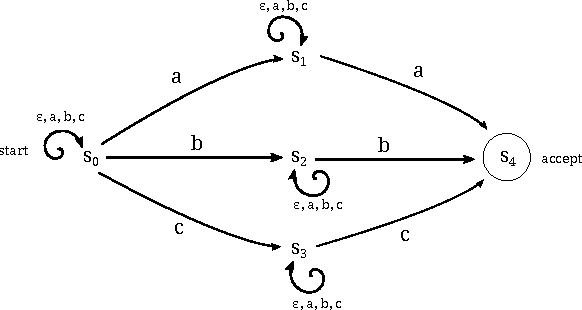
\includegraphics{resources/final-problem-1-nfa.pdf}
    \end{center}

(b) Put $r := \varepsilon + a + b + c$. Then the sought regular expression is
\[r^*ar^*a + r^*br^*b + r^*cr^*c.\]

\bigskip

\noindent 2. Show that the set of strings over \(\{0,1\}\) of the form $ww$ for some $w\in \{0,1\}^*$ is not a regular language.

\bigskip

\emph{Solution.} Write $L$ for the set in question and suppose for
contradiction that $L$ is regular. Then by the pumping lemma there exists $N >
0$ such that a given string $v = ww$ of length $> N$ may be decomposed as $v =
xyz$ with $xy^iz \in L$ for all $i \ge 0$ and $y \neq \varepsilon$ and $|xy|
\le N$. (This is the pumping lemma as stated in Hopcroft et al.) Let $$w_0 =
1\underbrace{00\cdots0}_{N}$$ be a 1 followed by $N$ zeros. Put $v_0 :=
w_0w_0$. Then $|v_0| = 2N+2 > N$ and the pumping lemma applies. For a word
$u\in \{0,1\}^*$ write $O(u) := \#\{\text{1's in } u\}$. Since $|xy| \le N <
|v_0|/2 = N+1$ it follows that $y$ can contain at most one of the 1's in $v_0$.
If $O(y) = 0$ then $xy^iz$ has the number of zeros before the middle 1 not
equal to the number of zeros after the middle one, and thus it cannot be of the
form $ww$ i.e.~cannot be in $L$. If $O(y)=1$ then for odd $i$, $xy^iz$ has an
odd number of ones and again it cannot be of the form $ww$.

\bigskip

\newcommand{\Mon}[1]{\ensuremath{\mathrm{Mon}\langle #1\rangle}}
\newcommand{\Grp}[1]{\ensuremath{\mathrm{Grp}\langle #1\rangle}}

\noindent 3. Let us recall some definitions. Let $X$ be a set and $\mathcal{R}$
be a subset of $X^*\times X^*$. We define \Mon{X|\mathcal{R}} to be the
quotient of $X^*$ modulo the congruence generated by $\mathcal{R}$. Let
$X^{\pm} := X\times \{1,-1\}$. We write $x$ or $x^1$ for $(x,1) \in X^\pm$ and
$x^{-1}$ for $(x,-1) \in X^\pm$. Put \[\mathcal{F}_X := \{(x^\alpha
x^{-\alpha}, \varepsilon) \in (X^\pm)^*\times (X^\pm)^* : x \in X, \alpha\in
\{1,-1\}\}\] and \[\Grp{X | \mathcal{S}} := \Mon{X^\pm | \mathcal{F}_X \cup
\mathcal{S}}.\] We also use the notation \(\Grp{x_1,\dots,x_s|U_1 = V_1, \dots,
U_t = V_t}\) to mean \Grp{X|\mathcal{S}} where $X = \{x_1,\dots,x_s\},
\mathcal{S} = \{(U_i,V_i)\}_{i=1}^t.$

Let $\mathbb{Z}$ be the additive group of integers and let $\mathbb{Z}/n$ be
the quotient by the subgroup $n\mathbb{Z}$.

Show that \Grp{x | x^n=1} is isomorphic to $\mathbb{Z}/n$.

\bigskip

\emph{Solution.} We define a map \(\mathbb{Z}\simeq
\{x,x^{-1}\}^*/\mathcal{F}_{\{x,x^{-1}\}}\rightarrow \mathbb{Z}/n\) by sending
$\varepsilon \mapsto 0, x\mapsto 1, x^{-1} \mapsto -1$. Here, the isomorphism
$\mathbb{Z}\simeq \{x,x^{-1}\}^*/\mathcal{F}_{\{x,x^{-1}\}}$ is just the fact
that $\{x,x^{-1}\}^*/\mathcal{F}_{\{x,x^{-1}\}}$ is the free group on one
generator, i.e.~$\mathbb{Z}$.

We now invoke the following proposition from the course notes.

\begin{prop} Let $M$ be a monoid and $Q$ be the quotient of $M$ mod the
    congruence $\sim$ generated by $S \subset M\times M$. Let $f: M \rightarrow
    N$ be a monoid homomorphism such that $f(s) = f(t)$ for all $(s,t)\in S$.
    Then there is a unique $g: Q \rightarrow N$ such that \[\xymatrix{ M
    \ar[rr]^f \ar[dr]_{x\mapsto [x]}& & N\\ & Q\ar[ur]_g } \] commutes.
\end{prop}

Thus we have a unique homomorphism of monoids $\Grp{x|x^n=1} \rightarrow
\mathbb{Z}/n$. Now we can write down a map $\mathbb{Z} \simeq
\{u,u^{-1}\}^*/\mathcal{F}_{\{u,u^{-1}\}} \rightarrow \Grp{x|x^n=1}$ by $u
\mapsto x$. Again we use the above proposition to get the monoid homomorphism
$\mathbb{Z}/n \rightarrow \Grp{x|x^n=1}$. One computes directly that the maps
are inverse (at this point, we have reduced to the intuitive proof from a first
course in group theory).

\bigskip

\noindent 4. Let $X$ be a set with at least two elements. Show that $X^*$ has
an infinite strictly increasing sequence of ideals.

\bigskip

\emph{Solution.} Recall that an ideal in a monoid $M$ is by definition a subset
$I \subset M$ such that $IM \subset I$ and $MI \subset I$. Let $a\in X$ are
distinct elements. For $n \ge 2$ put \[ I_n := \{w \in X^* : w(i) = w(j) = a
\text{ for some } 1 \le i < j \le n\}.\] One checks that the $I_n$ are ideals
and that we have \[I_2 \subsetneq I_3 \subsetneq \cdots\] as required. (Note
that if $X$ had only one element then all of the $I_n$ would coincide.)

\bigskip

\noindent 5. Draw a van Kampen diagram which shows that the group \[\langle a,b
| abab^2 = baba^2 = e\rangle\] is cyclic.

\bigskip

\emph{Solution.} In the diagram on the left, the pentagon is $abab^2=e$, the
outer boundary is $baba^2=e$ and the remaining bounded region is
$abb^{-1}b^{-1} = ab^{-1} = e$ so that $a=b$ and the group is cyclic. The
diagram on the right proceeds likewise.

    \begin{center}
        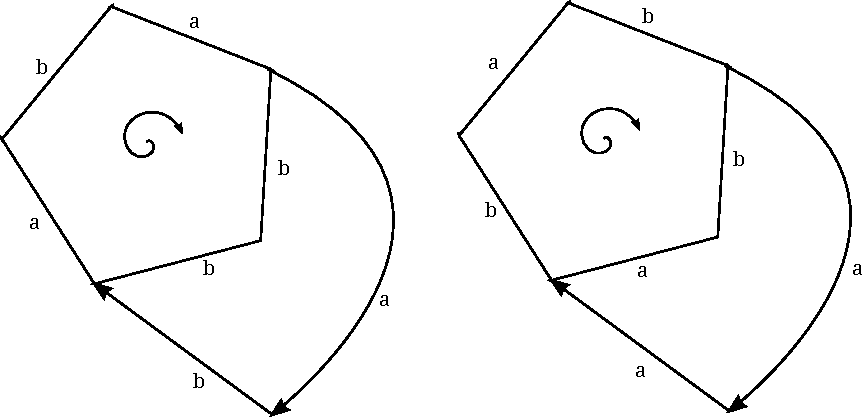
\includegraphics[scale=0.8]{resources/van-kampen-final.pdf}
    \end{center}

\bigskip

\noindent 6. Let $<$ be a reduction ordering on $X^*$ and let $\mathcal{R}$ be
a confluent rewriting system with respect to it. For a word $U\in X^*$ write
$U^\#$ for the reverse of $U$. Define $<^\#$ by $U <^\# V$ iff $U^\# < V^\#$.

(a) Show that $<^\#$ is a reduction ordering.

(b) Show that $\{(P^\#,Q^\#) : (P,Q)\in \mathcal{R}\}$ is a confluent rewriting
system with respect to $<^\#$.

\bigskip

\emph{Solution.} (a) Given $U,V$ we must show that $U <^\# V \Rightarrow AUB
<^\# AVB$ for all $A,B$. The latter holds iff $(AUB)^\# = B^\# U^\# A^\# <
(AVB)^\# = B^\# V^\# A^\#$. Now this last condition does hold since $<$ is
translation invariant and $U^\# < V^\#.$ Thus $<^\#$ is translation invariant.

To see that it is a well ordering suppose not; then there is an infinite
strictly decreasing sequence $U_1^\# > U_2^\# > \cdots$ contradicting the fact
that $<$ is a well ordering.

(b) Unwind the definitions. (Note: the students were required to write out a
detailed proof to receive full credit.)

\bigskip

\noindent 7. Let $X := \{x,y,z\}$ and consider the finite rewriting system
$$\mathcal{R} := \{(x^2, \varepsilon),\; (yz, \varepsilon),\; (zy,\varepsilon)
\}.$$ Show that $\mathcal{R}$ is confluent.

\bigskip

\emph{Solution.}

Let us first recall the idea behind the algorithm \textsc{Confluent}.

We have the following proposition from the course notes:

\begin{prop} Let $W$ be a word such that local confluence fails at $W$ but does
    not fail at any proper subword of $W$. Then one of the following holds:

    (1) $W$ appears as the left side of two distinct elements of $\mathcal{R}$.

    (2) $W$ is a left side in $\mathcal{R}$ which contains another left side as a proper subword.

    (3) $W = ABC$ where $A,B,C$ are nonempty words such that $AB$ and $BC$ are left sides in $\mathcal{R}$.
\end{prop}

\begin{defn} If $W$ is as in the proposition, then we call $W$ an \emph{overlap
    of left sides} in $\mathcal{R}$. If the third condition holds then we say
    that $W$ is a \emph{proper overlap.}
\end{defn}

Since $\mathcal{R}$ is finite, the set $\mathscr{W}$ of words which are
overlaps of left sides in $\mathcal{R}$ is also finite. For each $W\in
\mathscr{W}$, write $\mathscr{U}$ for the finite set of words $U$ such that $W
\xrightarrow{\mathcal{R}} U$ is a derivation consisting of a single step. For
each $U\in \mathscr{U}$ we put $V :=$ \textsc{Rewrite}$(X,\mathcal{R},U)$.  As
$U$ varies, if more than one $V$ is obtained, then $\mathcal{R}$ is not
confluent. The reason is that in this case we have found two words which are
irreducible with respect to $\mathcal{R}$ and define the same element of $M$.

On the other hand, if only one value of $V$ is seen as $U$ varies in
$\mathscr{U}$, then local confluence does not fail at $W$.

Performing this test for all $W\in \mathscr{W}$, we have an algorithm
\textsc{Confluent} for determining whether or not $\mathcal{R}$ is confluent.

Now, to solve the problem at hand, we must first determine $\mathscr{W}$. Cases
(1) and (2) of the proposition do not arise. For case (3): corresponding to
$(x^2, \varepsilon)$ we have $A=x, B=x, C=x$ in the notation of the
proposition, so that $W = ABC$ with $AB = BC = x^2$ a left side. If we take
$A=y, B=z, C=y$ then we have $AB=yz, BC=zy$ are left sides so that $W=ABC=yzy$
is in $\mathscr{W}$. Similarly if we take $A=z, B=y, C=z$ then $AB=zy, BC=yz$
are left sides and it follows that $W = zyz \in \mathscr{W}$. This exhausts all
possible elements of $\mathscr{W}$ since we have checked all left sides for
candidates for $AB,BC$ and $A,B,C$.

Now, $\mathscr{W} = \{x^3, yzy, zyz\}$. Fix $W\in \mathscr{W}$. We must find
the set $\mathscr{U}_W$ of words that can be obtained in one step from $W$.
Inspecting $\mathcal{R}$ we see that $$\mathscr{U}_{x^3} = \{x\},\;\;
\mathscr{U}_{yzy} = \{y\},\;\; \mathscr{U}_{zyz} = \{z\}.$$ Finally, for each
$W\in \mathscr{W}$ we see that the set $$\{
\text{\textsc{Rewrite}}(X,\mathcal{R},U) : U \in \mathscr{U}_W\}$$ is a
singleton, a fact which verifies confluence.

\bigskip

\noindent 8. Let us recall the Knuth-Bendix algorithm and the supporting subroutines, as well as the Euclidean algorithm.

\bigskip

\begin{algorithmic}[1]
    \Procedure{RewriteLeft}{$X,\mathcal{R}, U$}
    \State Input: $X$ = generators, $\mathcal{R}$ = rewriting system, $U$ = a word;
    \State Output: the rewritten form of $U$
    \State $V:= \varepsilon, W := U$;
    \While{$W \neq \varepsilon$}
    \State Let $W = xW_1$ where $x\in X$; $W:= W_1, V:= Vx;$
    \For{$i = 1,\dots,n$}
    \If{$P_i$ is a suffix of $V$}
    \State $V:= RP_i, W := Q_i W, V:= R;$
    \State break
    \EndIf
    \EndFor
    \EndWhile
    \EndProcedure
\end{algorithmic}

\bigskip

\begin{algorithmic}[1]
    \Procedure{Update}{$\mathcal{S}, U,V$}
    \State Input: $\mathcal{S} = \{(P_1,Q_1), (P_2,Q_2), \dots,(P_n,Q_n)\}$ a finite rewriting system; $U,V = $ words;
    \State Output: none; the state of $\mathcal{S}$ is modified in place;
    \State $A :=$ \textsc{RewriteLeft}$(U)$;
    \State $B :=$ \textsc{RewriteLeft}$(V)$;
    \If{$A\neq B$}
    \If{$A < B$}
    \State swap $A$ and $B$;
    \EndIf
    \State append $(A,B)$ to $\mathcal{S}$;
    \EndIf
    \EndProcedure
\end{algorithmic}

\bigskip

\begin{algorithmic}[1]
    \Procedure{Overlap}{$\mathcal{S}, i,j$}
    \State Input: $\mathcal{S} = \{(P_1,Q_1), (P_2,Q_2), \dots,(P_n,Q_n)\}$; $i,j = $ positive integers $\le |\mathcal{S}|$
    \State Output: none; the state of $\mathcal{S}$ is modified in place;
    \For{$k := 1, \dots, |P_i|$}
    \State Let $P_i = AB$ where $|B| = k$;
    \State Let $U$ be the longest word which is a prefix of both $B$ and $P_j$;
    \State Let $B = UD$ and $P_j = UE;$
    \If{$D = \varepsilon$ or $E = \varepsilon$}
    \State \textsc{Update}$(\mathcal{S}, AQ_jD, Q_iE)$;
    \EndIf
    \EndFor
    \EndProcedure
\end{algorithmic}

\bigskip

\begin{algorithmic}[1]
    \Procedure{KnuthBendix}{$X, <, \mathcal{R}$}
    \State Input:
    \State $X=$ a finite set, $<$ = reduction ordering on $X^*$, $\mathcal{R} \subset X^*\times X^*$ a finite subset;
    \State Output: $\mathcal{T} = \mathrm{RC}(X, <, \mathcal{R})$ if it is finite
    \State
    \State $\mathcal{S} := \{\};i:=1;$
    \For{$(U,V) \in \mathcal{R}$}
    \State \textsc{Update}$(\mathcal{S},U,V);$
    \EndFor
    \While{$i \le n$}
    \For{$j:=1,\dots,i$}
    \State \textsc{Overlap}$(\mathcal{S}, i,j)$;
    \If{j < i}
    \State \textsc{Overlap}$(\mathcal{S}, j,i)$;
    \EndIf
    \EndFor
    \State $i := i+1;$
    \EndWhile
    \State Let $\mathcal{P} := \{P_i : \text{every proper subword of } P_i \text{ is irreducible wrt } \mathcal{S}\}$;
    \State $\mathcal{T} := \{\}$;
    \For{$P\in \mathcal{P}$}
    \State $Q :=$ \textsc{RewriteLeft}$(X, \mathcal{R}, P)$;
    \State append $(P,Q)$ to $\mathcal{T}$;
    \EndFor
    \EndProcedure
\end{algorithmic}

\bigskip
\noindent The following is the Euclidean algorithm for positive integers $a,b$:

\bigskip

\begin{algorithmic}[1]
    \Procedure{gcd}{a,b}
    \If{$a = 0$}
    \State return $b$
    \EndIf
    \While{$b \neq 0$}
    \If{$a > b$}
    \State $a := a-b$
    \Else
    \State $b := b-a$
    \EndIf
    \EndWhile
    \State return $a$
    \EndProcedure
\end{algorithmic}

\bigskip

Let $X=\{x\}$ and let $$\mathcal{R} := \{x^m\rightarrow \varepsilon,\;\;
x^n\rightarrow \varepsilon\}$$ where $m,n \in \mathbb{Z}_{>0}$.

Show that the Knuth-Bendix algorithm returns a confluent rewriting system
consisting of the single rule \[x^{\mathrm{gcd}(m,n)} \rightarrow
\varepsilon.\] In writing your proof, refer to the line numbers given in the
above code. In the course of your proof, compare the execution of
$\mathrm{gcd}(m,n)$ using the Euclidean algorithm with the execution of the
Knuth-Bendix algorithm.

\bigskip

\emph{Solution.} Suppose without loss that $m>n$. Line 7-8 of
\textsc{KnuthBendix} starts us off with $\mathcal{S} =
\{(x^m,\varepsilon),(x^n,\varepsilon)\}$ and then line 12 of
\textsc{KnuthBendix} gives rise to an \textsc{Update} call in line 9 of
\textsc{Overlap}. This appends $(x^{m-n},\varepsilon)$ to $\mathcal{S}$,
corresponding to line 7 of the gcd algorithm. The successive calls to
\textsc{Overlap} lines 12 and 14 (and the resulting calls to \textsc{Update} in
line 9 of \textsc{Overlap}) of \textsc{KnuthBendix} correspond to lines 7 and 9
of gcd.

A much more in depth discussion of the similarities between the Knuth-Bendix
algorithm and the Gr\"obner-Buchberger algorithm (of which the gcd is the basic
example) may be found in the paper ``Algebraic Simplification'' by Buchberger
and Loos (1982).

\bigskip

\noindent 9. Given \(w \in \{0,1\}^*\) we write $w = a_n a_{n-1} \cdots a_0$
with $a_i \in \{0,1\}$ for all $i$. We define $\mathrm{eval}(w) := \sum_{i=0}^n
a_i2^i$. Thus $\mathrm{eval} : \{0,1\}^* \rightarrow \mathbb{Z}_{\ge 0}$ is a
well defined function. In other words, using the eval function, we regard $w$
as representing a nonnegative integer written in base 2 in the usual way.

Show that the language \[\mathscr{L} := \{w \in \{0,1\}^* : w \text{ starts
with a } 1 \text{ and } \mathrm{eval}(w) \text{ is a prime number}\}\] is not
regular.

\bigskip

\emph{Solution.} This was a challenge problem. None of the students could solve
it on the exam. The the solution is on page 57 of Analytic Combinatorics by
Flajolet and Sedgewick.
\end{document}
